

\begin{figure}[H] \caption{Number of Children in Preschool in Reggio Emilia} \label{fig:num-children-RE}
	\centering
	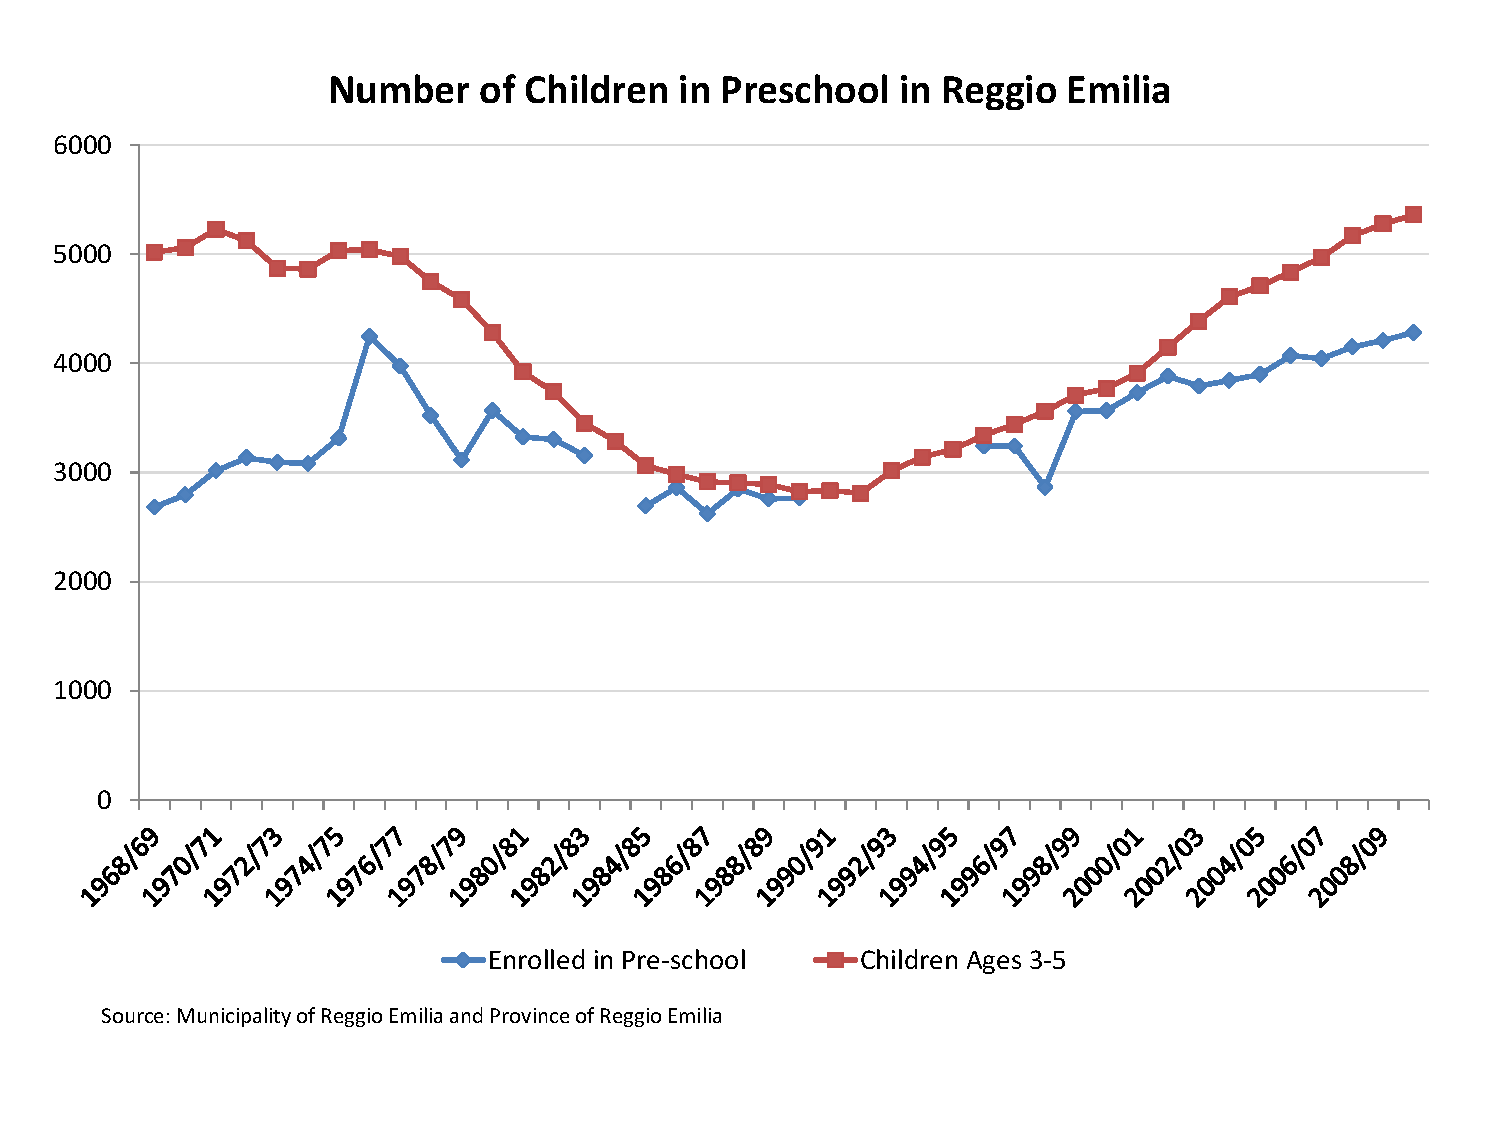
\includegraphics[scale=0.65]{../../output/image/Enrollement_Preschool_RE.pdf}
\end{figure}

Figure \ref{fig:num-children-RE} shows the number of children in preschool in Reggio Emilia. The gap in figure shows that data is not available for the corresponding years. It is shown that the percentage of children enrolled in preschool increases over the period from 1968 to 2000. After-2000, the percentage of children decreases again according to the data we use. 

%\begin{figure}[H] \caption{Number of Children in Preschool in Padova} \label{fig:num_children_Pv}
%	\centering
%	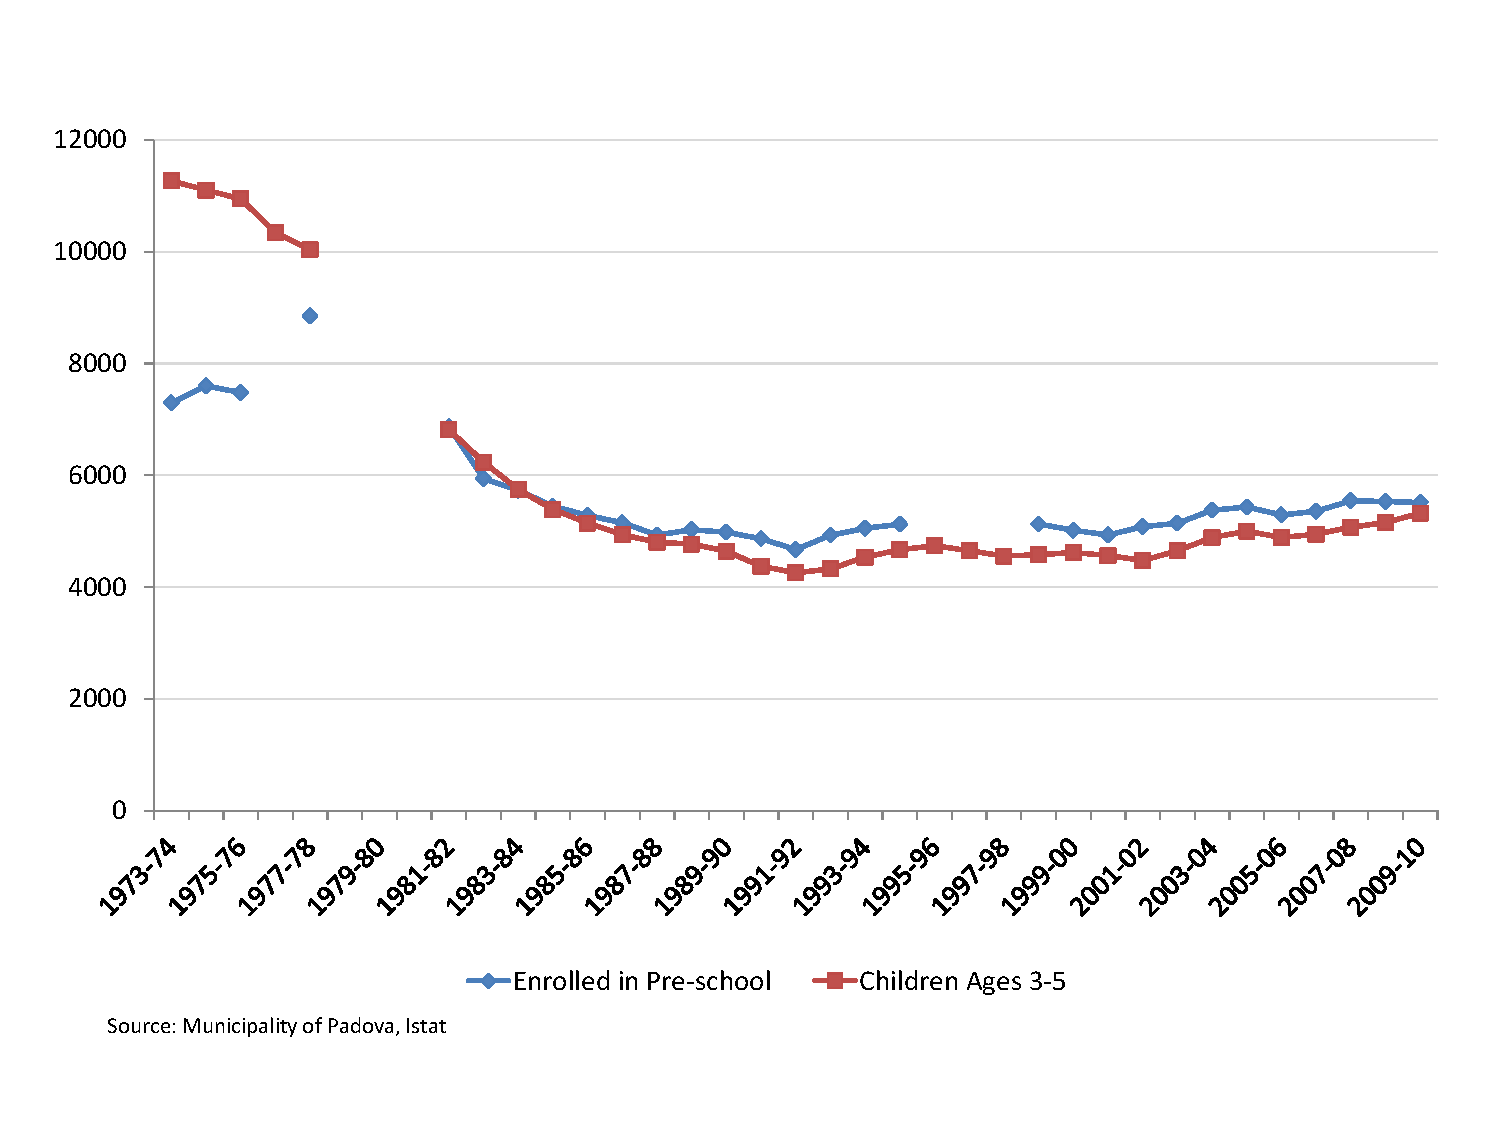
\includegraphics[scale=0.65]{../../output/image/Enrollement_Preschool_Padova.pdf}
%\end{figure}

%Figure \ref{fig:num_children_Pv} shows the number of children in preschool in Padova. The gap in figure shows that data is not available for the corresponding years. It is shown that the percentage of children enrolled in preschool increases over time. 


%\begin{figure}[H] \caption{Enrolled in Preschool as Percent of Children Ages 3-5} \label{fig:enroll-pres-3-5}
%	\centering
%	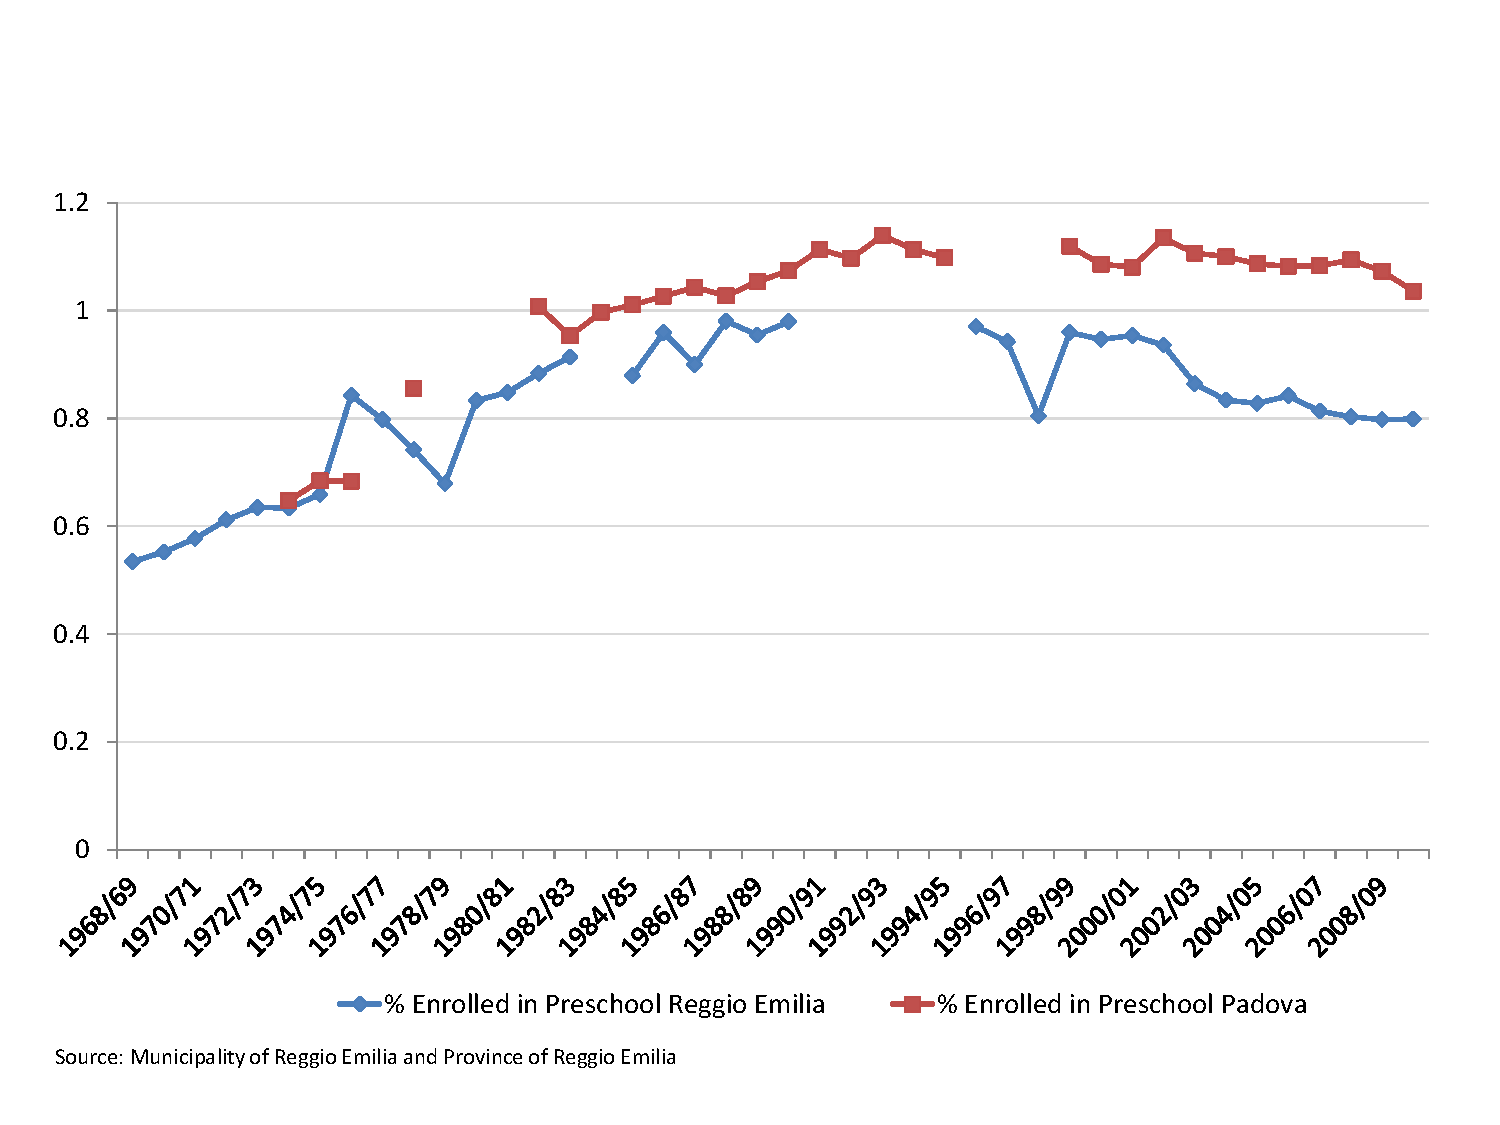
\includegraphics[scale=0.65]{../../output/image/Enrollement_Preschool_age3-5.pdf}
%\end{figure}

%Figure \ref{fig:enroll-pres-3-5} shows the enrollment in preschool as percentage of children of ages 3-5. The gap in figure shows that data is not available for the corresponding years. It is shown that The enrollment rate in Padova generally exceeds the rate in Reggio Emilia. 